% tikz flowchart
\begin{figure}[H]
\centering

\tikzset{every picture/.style={line width=0.75pt}} %set default line width to 0.75pt        

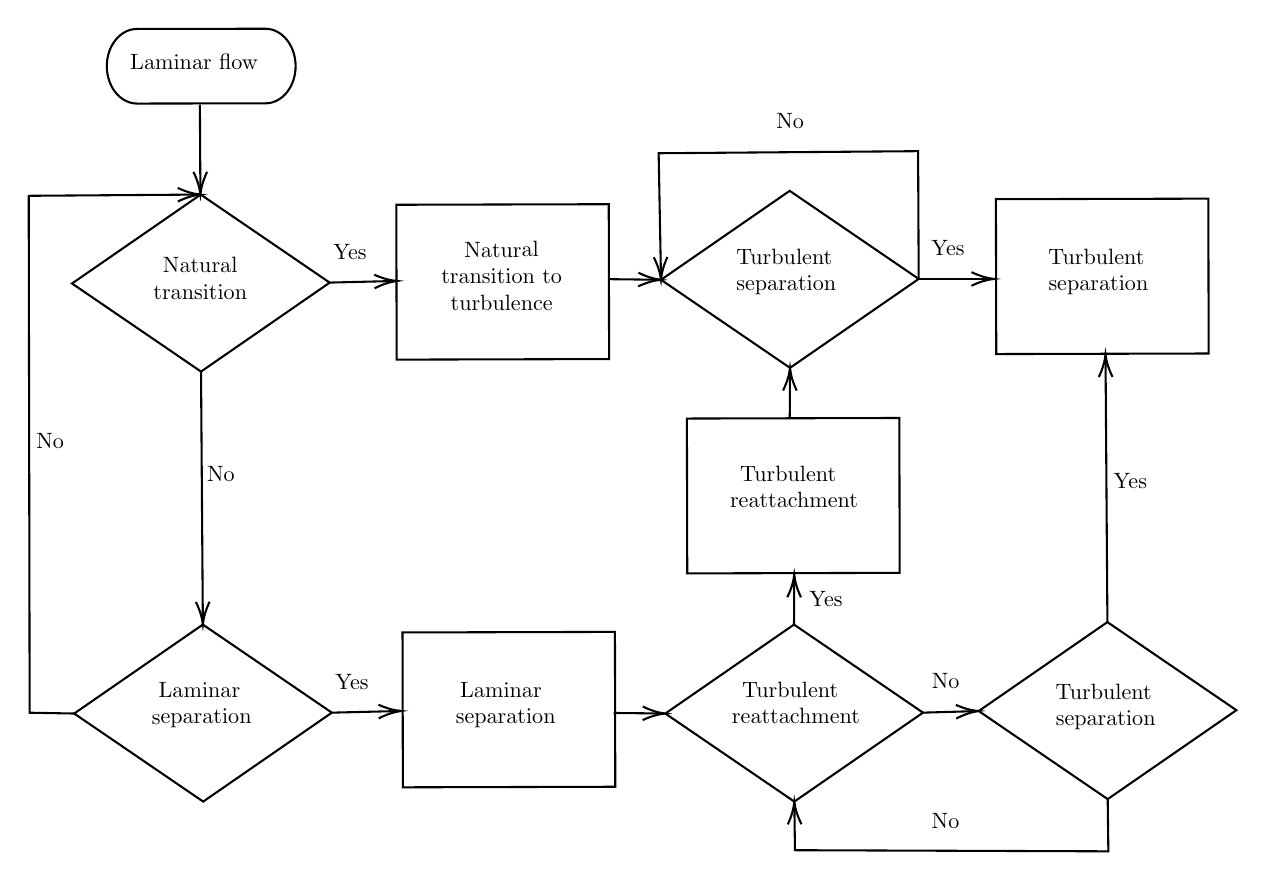
\begin{tikzpicture}[x=0.75pt,y=0.75pt,yscale=-1,xscale=1]
%uncomment if require: \path (0,734); %set diagram left start at 0, and has height of 734

%Flowchart: Terminator [id:dp7207071910268746] 
\draw   (68.63,154.62) -- (130.49,154.51) .. controls (138.52,154.5) and (145.06,162.53) .. (145.09,172.46) .. controls (145.12,182.38) and (138.62,190.44) .. (130.59,190.45) -- (68.73,190.56) .. controls (60.7,190.57) and (54.16,182.54) .. (54.13,172.61) .. controls (54.1,162.69) and (60.6,154.63) .. (68.63,154.62) -- cycle ;
%Straight Lines [id:da10986730772092312] 
\draw    (98.97,191.03) -- (99.21,232.4) ;
\draw [shift={(99.22,234.4)}, rotate = 269.67] [color={rgb, 255:red, 0; green, 0; blue, 0 }  ][line width=0.75]    (10.93,-3.29) .. controls (6.95,-1.4) and (3.31,-0.3) .. (0,0) .. controls (3.31,0.3) and (6.95,1.4) .. (10.93,3.29)   ;
%Straight Lines [id:da11218528639690684] 
\draw    (99.52,319.69) -- (100.39,439.58) ;
\draw [shift={(100.41,441.58)}, rotate = 269.58] [color={rgb, 255:red, 0; green, 0; blue, 0 }  ][line width=0.75]    (10.93,-3.29) .. controls (6.95,-1.4) and (3.31,-0.3) .. (0,0) .. controls (3.31,0.3) and (6.95,1.4) .. (10.93,3.29)   ;
%Flowchart: Decision [id:dp47636663676641755] 
\draw   (100.41,441.58) -- (162.55,484.02) -- (100.56,526.87) -- (38.41,484.44) -- cycle ;
%Flowchart: Process [id:dp0035186106511891913] 
\draw   (193.61,239.32) -- (295.96,239.05) -- (296.13,313.66) -- (193.78,313.93) -- cycle ;
%Straight Lines [id:da41405154544556755] 
\draw    (160.52,276.84) -- (191.97,276.07) ;
\draw [shift={(193.97,276.03)}, rotate = 538.61] [color={rgb, 255:red, 0; green, 0; blue, 0 }  ][line width=0.75]    (10.93,-3.29) .. controls (6.95,-1.4) and (3.31,-0.3) .. (0,0) .. controls (3.31,0.3) and (6.95,1.4) .. (10.93,3.29)   ;
%Straight Lines [id:da4839414628019604] 
\draw    (38.41,484.44) -- (16.95,484.05) -- (16.5,235) -- (97.22,234.42) ;
\draw [shift={(99.22,234.4)}, rotate = 539.5899999999999] [color={rgb, 255:red, 0; green, 0; blue, 0 }  ][line width=0.75]    (10.93,-3.29) .. controls (6.95,-1.4) and (3.31,-0.3) .. (0,0) .. controls (3.31,0.3) and (6.95,1.4) .. (10.93,3.29)   ;
%Straight Lines [id:da47695648438676885] 
\draw    (296.33,275.17) -- (319.14,275.44) ;
\draw [shift={(321.14,275.47)}, rotate = 180.69] [color={rgb, 255:red, 0; green, 0; blue, 0 }  ][line width=0.75]    (10.93,-3.29) .. controls (6.95,-1.4) and (3.31,-0.3) .. (0,0) .. controls (3.31,0.3) and (6.95,1.4) .. (10.93,3.29)   ;
%Flowchart: Decision [id:dp5291766920258706] 
\draw   (99.37,234.4) -- (161.52,276.84) -- (99.52,319.69) -- (37.37,277.25) -- cycle ;
%Flowchart: Process [id:dp6243738863575946] 
\draw   (196.6,445.38) -- (298.94,445.11) -- (299.11,519.72) -- (196.77,519.99) -- cycle ;
%Flowchart: Process [id:dp6109994002876044] 
\draw   (482.49,236.64) -- (584.83,236.37) -- (585,310.98) -- (482.66,311.25) -- cycle ;
%Flowchart: Decision [id:dp19310726941760736] 
\draw   (383.14,232.61) -- (445.29,275.05) -- (383.29,317.9) -- (321.14,275.46) -- cycle ;
%Flowchart: Decision [id:dp374284511592351] 
\draw   (536.21,440.39) -- (598.35,482.83) -- (536.35,525.68) -- (474.21,483.24) -- cycle ;
%Flowchart: Decision [id:dp9780902027233841] 
\draw   (385.22,441.58) -- (447.37,484.02) -- (385.37,526.87) -- (323.22,484.44) -- cycle ;
%Straight Lines [id:da6310642789542652] 
\draw    (162.55,484.02) -- (194.01,483.26) ;
\draw [shift={(196.01,483.21)}, rotate = 538.61] [color={rgb, 255:red, 0; green, 0; blue, 0 }  ][line width=0.75]    (10.93,-3.29) .. controls (6.95,-1.4) and (3.31,-0.3) .. (0,0) .. controls (3.31,0.3) and (6.95,1.4) .. (10.93,3.29)   ;
%Straight Lines [id:da12370255545736619] 
\draw    (445.29,275.05) -- (479.66,275.05) ;
\draw [shift={(481.66,275.05)}, rotate = 180] [color={rgb, 255:red, 0; green, 0; blue, 0 }  ][line width=0.75]    (10.93,-3.29) .. controls (6.95,-1.4) and (3.31,-0.3) .. (0,0) .. controls (3.31,0.3) and (6.95,1.4) .. (10.93,3.29)   ;
%Straight Lines [id:da6933448349630812] 
\draw    (298.33,484.17) -- (321.22,484.41) ;
\draw [shift={(323.22,484.44)}, rotate = 180.62] [color={rgb, 255:red, 0; green, 0; blue, 0 }  ][line width=0.75]    (10.93,-3.29) .. controls (6.95,-1.4) and (3.31,-0.3) .. (0,0) .. controls (3.31,0.3) and (6.95,1.4) .. (10.93,3.29)   ;
%Straight Lines [id:da4268759513220136] 
\draw    (445.29,275.05) -- (445,213.5) -- (320,214.5) -- (321.11,273.47) ;
\draw [shift={(321.14,275.47)}, rotate = 268.93] [color={rgb, 255:red, 0; green, 0; blue, 0 }  ][line width=0.75]    (10.93,-3.29) .. controls (6.95,-1.4) and (3.31,-0.3) .. (0,0) .. controls (3.31,0.3) and (6.95,1.4) .. (10.93,3.29)   ;
%Straight Lines [id:da994392836584868] 
\draw    (447.37,484.02) -- (472.21,483.3) ;
\draw [shift={(474.21,483.24)}, rotate = 538.3199999999999] [color={rgb, 255:red, 0; green, 0; blue, 0 }  ][line width=0.75]    (10.93,-3.29) .. controls (6.95,-1.4) and (3.31,-0.3) .. (0,0) .. controls (3.31,0.3) and (6.95,1.4) .. (10.93,3.29)   ;
%Straight Lines [id:da7889844522327492] 
\draw    (536.35,525.68) -- (536.67,550.83) -- (385.67,550.29) -- (385.4,528.87) ;
\draw [shift={(385.37,526.87)}, rotate = 449.27] [color={rgb, 255:red, 0; green, 0; blue, 0 }  ][line width=0.75]    (10.93,-3.29) .. controls (6.95,-1.4) and (3.31,-0.3) .. (0,0) .. controls (3.31,0.3) and (6.95,1.4) .. (10.93,3.29)   ;
%Straight Lines [id:da8600462573826505] 
\draw    (536.21,440.39) -- (535.31,313.33) ;
\draw [shift={(535.3,311.33)}, rotate = 449.6] [color={rgb, 255:red, 0; green, 0; blue, 0 }  ][line width=0.75]    (10.93,-3.29) .. controls (6.95,-1.4) and (3.31,-0.3) .. (0,0) .. controls (3.31,0.3) and (6.95,1.4) .. (10.93,3.29)   ;
%Flowchart: Process [id:dp7123966290133054] 
\draw   (333.61,342.32) -- (435.96,342.05) -- (436.13,416.66) -- (333.78,416.93) -- cycle ;
%Straight Lines [id:da1825292614199847] 
\draw    (383.17,342) -- (383.28,319.9) ;
\draw [shift={(383.29,317.9)}, rotate = 450.29] [color={rgb, 255:red, 0; green, 0; blue, 0 }  ][line width=0.75]    (10.93,-3.29) .. controls (6.95,-1.4) and (3.31,-0.3) .. (0,0) .. controls (3.31,0.3) and (6.95,1.4) .. (10.93,3.29)   ;
%Straight Lines [id:da8063640644778529] 
\draw    (385.22,441.58) -- (385.33,419.49) ;
\draw [shift={(385.34,417.49)}, rotate = 450.29] [color={rgb, 255:red, 0; green, 0; blue, 0 }  ][line width=0.75]    (10.93,-3.29) .. controls (6.95,-1.4) and (3.31,-0.3) .. (0,0) .. controls (3.31,0.3) and (6.95,1.4) .. (10.93,3.29)   ;

% Text Node
\draw (162.01,257.44) node [anchor=north west][inner sep=0.75pt]  [rotate=-359.86,xscale=0.8,yscale=0.8] [align=left] {{\normalsize Yes}};
% Text Node
\draw (101.21,364.24) node [anchor=north west][inner sep=0.75pt]  [rotate=-359.86,xscale=0.8,yscale=0.8] [align=left] {{\normalsize No}};
% Text Node
\draw (450.19,255.43) node [anchor=north west][inner sep=0.75pt]  [rotate=-359.86,xscale=0.8,yscale=0.8] [align=left] {{\normalsize Yes}};
% Text Node
\draw (18.92,348.42) node [anchor=north west][inner sep=0.75pt]  [rotate=-359.86,xscale=0.8,yscale=0.8] [align=left] {{\normalsize No}};
% Text Node
\draw (356.18,254.04) node [anchor=north west][inner sep=0.75pt]  [rotate=-359.86,xscale=0.8,yscale=0.8] [align=left] {\begin{minipage}[lt]{43.095000000000006pt}\setlength\topsep{0pt}
\begin{center}
{\normalsize Turbulent \ }\\{\normalsize separation }
\end{center}

\end{minipage}};
% Text Node
\draw (64.2,165.4) node [anchor=north west][inner sep=0.75pt]  [font=\normalsize,rotate=-360,xscale=0.8,yscale=0.8] [align=left] {{\normalsize Laminar flow}};
% Text Node
\draw (65.17,263.54) node [anchor=north west][inner sep=0.75pt]  [font=\normalsize,rotate=-359.86,xscale=0.8,yscale=0.8] [align=left] {\begin{minipage}[lt]{61.34875pt}\setlength\topsep{0pt}
\begin{center}
{\normalsize Natural transition }\\
\end{center}

\end{minipage}};
% Text Node
\draw (74.55,468.21) node [anchor=north west][inner sep=0.75pt]  [rotate=-359.86,xscale=0.8,yscale=0.8] [align=left] {\begin{minipage}[lt]{43.095000000000006pt}\setlength\topsep{0pt}
\begin{center}
{\normalsize Laminar}\\{\normalsize separation }
\end{center}

\end{minipage}};
% Text Node
\draw (209.74,255.99) node [anchor=north west][inner sep=0.75pt]  [rotate=-359.86,xscale=0.8,yscale=0.8] [align=left] {\begin{minipage}[lt]{62.591875pt}\setlength\topsep{0pt}
\begin{center}
{\normalsize Natural transition to}\\{\normalsize turbulence}
\end{center}

\end{minipage}};
% Text Node
\draw (221.02,468.11) node [anchor=north west][inner sep=0.75pt]  [rotate=-359.86,xscale=0.8,yscale=0.8] [align=left] {\begin{minipage}[lt]{40.831875000000004pt}\setlength\topsep{0pt}
\begin{center}
{\normalsize Laminar }\\{\normalsize separation}
\end{center}

\end{minipage}};
% Text Node
\draw (162.99,464.51) node [anchor=north west][inner sep=0.75pt]  [rotate=-359.86,xscale=0.8,yscale=0.8] [align=left] {{\normalsize Yes}};
% Text Node
\draw (506.57,254.06) node [anchor=north west][inner sep=0.75pt]  [rotate=-359.86,xscale=0.8,yscale=0.8] [align=left] {\begin{minipage}[lt]{41.426875pt}\setlength\topsep{0pt}
\begin{center}
{\normalsize Turbulent \ }\\{\normalsize separation}
\end{center}

\end{minipage}};
% Text Node
\draw (354.14,467.97) node [anchor=north west][inner sep=0.75pt]  [rotate=-360,xscale=0.8,yscale=0.8] [align=left] {\begin{minipage}[lt]{52.615pt}\setlength\topsep{0pt}
\begin{center}
{\normalsize Turbulent \ }\\{\normalsize reattachment }\\
\end{center}

\end{minipage}};
% Text Node
\draw (375.51,194.09) node [anchor=north west][inner sep=0.75pt]  [rotate=-359.86,xscale=0.8,yscale=0.8] [align=left] {{\normalsize No}};
% Text Node
\draw (510.09,463.57) node [anchor=north west][inner sep=0.75pt]  [rotate=-359.86,xscale=0.8,yscale=0.8] [align=left] {\begin{minipage}[lt]{43.095000000000006pt}\setlength\topsep{0pt}
\begin{center}
{\normalsize Turbulent }\\{\normalsize separation }
\end{center}

\end{minipage}};
% Text Node
\draw (450.33,531.37) node [anchor=north west][inner sep=0.75pt]  [rotate=-359.86,xscale=0.8,yscale=0.8] [align=left] {{\normalsize No}};
% Text Node
\draw (391.35,424.48) node [anchor=north west][inner sep=0.75pt]  [rotate=-359.86,xscale=0.8,yscale=0.8] [align=left] {{\normalsize Yes}};
% Text Node
\draw (450.37,464.05) node [anchor=north west][inner sep=0.75pt]  [rotate=-359.86,xscale=0.8,yscale=0.8] [align=left] {{\normalsize No}};
% Text Node
\draw (538.01,367.44) node [anchor=north west][inner sep=0.75pt]  [rotate=-359.86,xscale=0.8,yscale=0.8] [align=left] {{\normalsize Yes}};
% Text Node
\draw (353.14,363.97) node [anchor=north west][inner sep=0.75pt]  [rotate=-359.86,xscale=0.8,yscale=0.8] [align=center] {\begin{minipage}[lt]{52.615pt}\setlength\topsep{0pt}
\begin{center}
{\normalsize Turbulent \ }\\{\normalsize reattachment }\\
\end{center}

\end{minipage}};


\end{tikzpicture}

\caption{Boundary layer flowchart} 
\label{fig:Boundary layer flowchart}
\end{figure}


\pagebreak

% listing of script
\lstinputlisting[style= Matlab-editor,basicstyle = \mlttfamily,
  caption=Exercise 6 script]{Week_2_master/exercise6.m}

% four plots as specified
\begin{figure}[H]
\centering
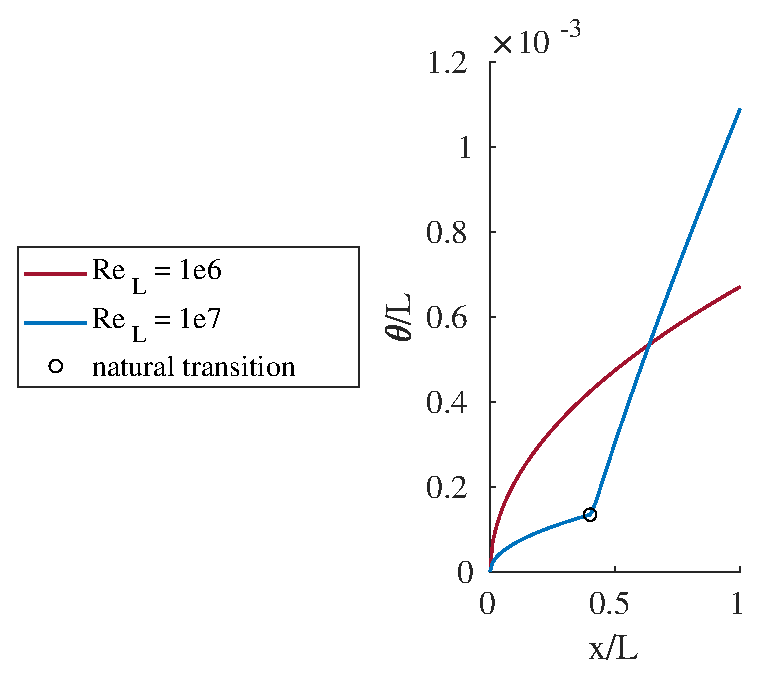
\includegraphics[scale=0.8]{graphs/e6g1.eps}
\caption{Momentum thickness plot for $Re_l = 10^6$ and $10^7$ for zero velocity gradient}
\label{e6g1}
\end{figure}

\begin{figure}[H]
\centering
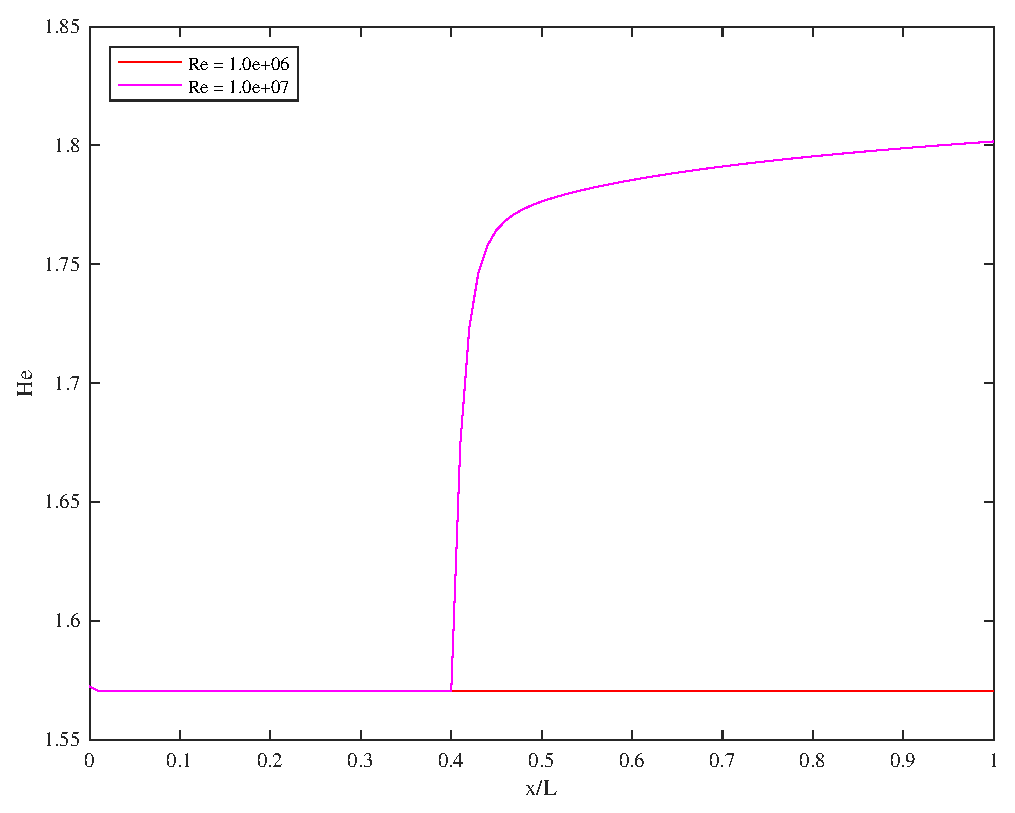
\includegraphics[scale=0.8]{graphs/e6g2.eps}
\caption{Energy thickness plot for $Re_l = 10^6$ and $10^7$ for zero velocity gradient}
\label{e6g2}
\end{figure}

\begin{figure}[H]
\centering
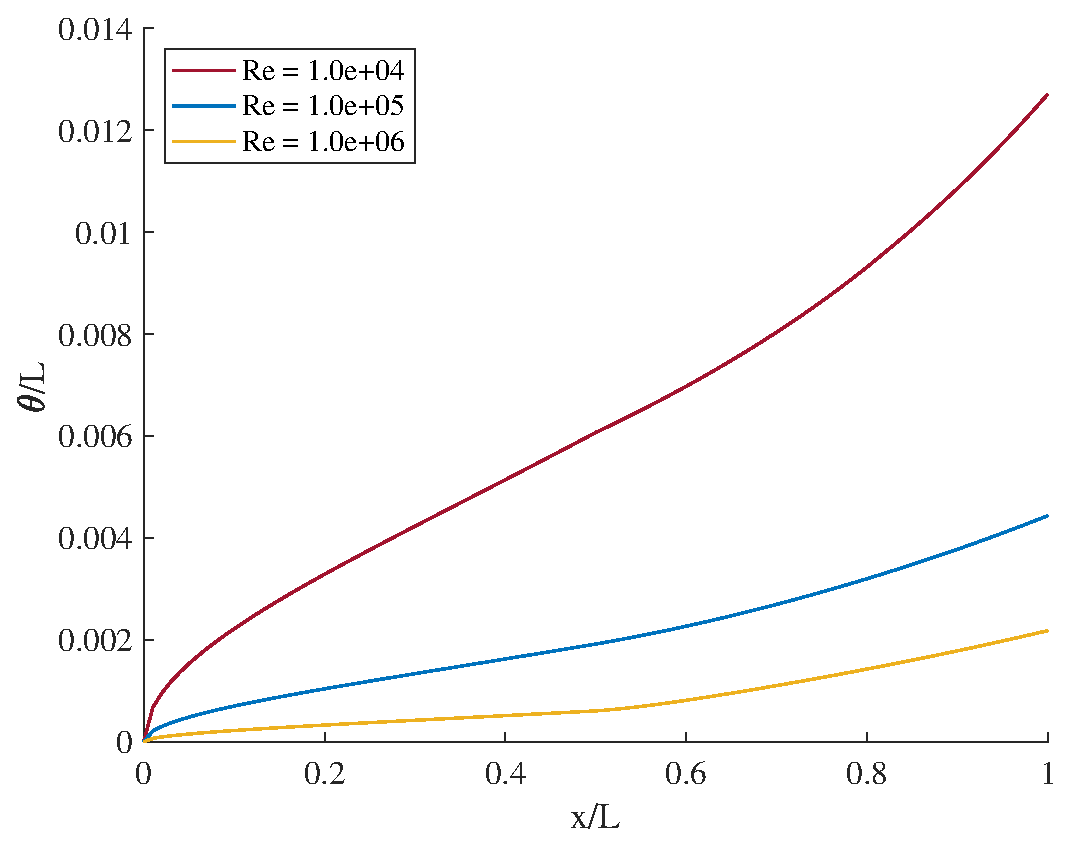
\includegraphics[scale=0.8]{graphs/e6g3.eps}
\caption{Momentum thickness plot for $Re_l = 10^4, 10^5$ and $10^6$ for velocity gradient = -0.25}
\label{e6g3}
\end{figure}

\begin{figure}[H]
\centering
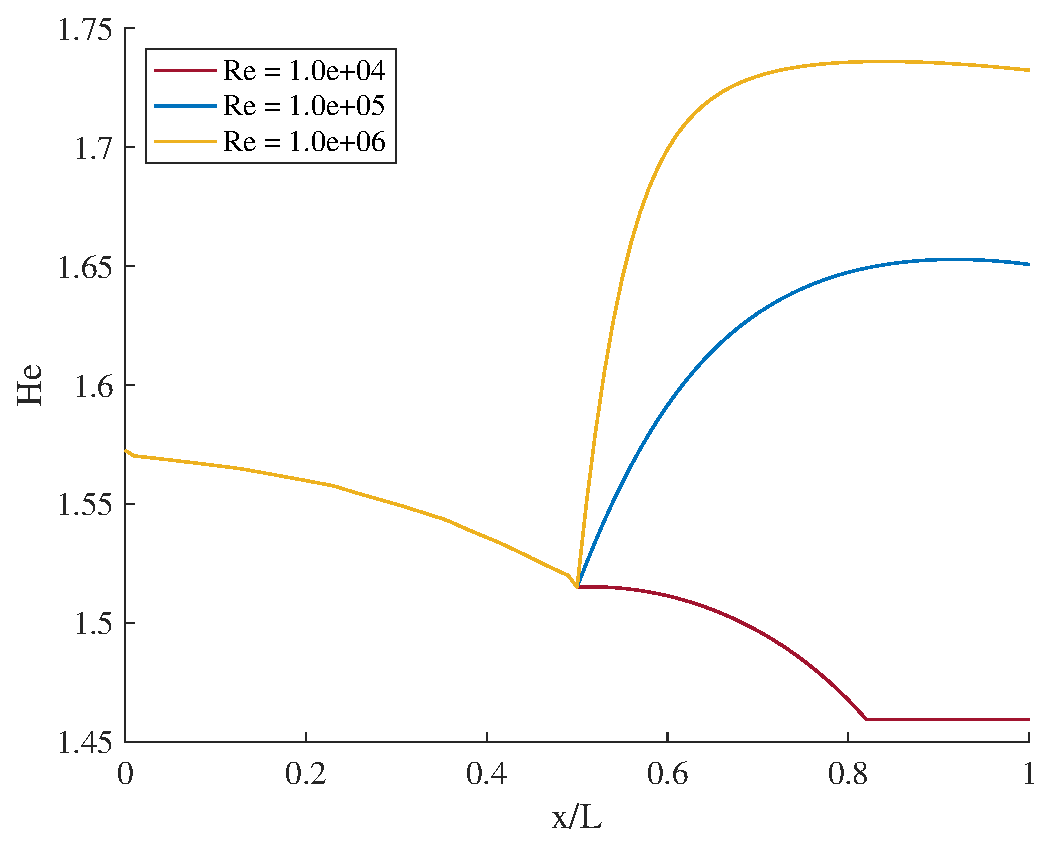
\includegraphics[scale=0.8]{graphs/e6g4.eps}
\caption{Energy thickness plot for $Re_l = 10^4, 10^5$ and $10^6$ for velocity gradient = -0.25}
\label{e6g4}
\end{figure}

\pagebreak

% critical velocity gradient as specified
\lstinputlisting[style= Matlab-editor,basicstyle = \mlttfamily,
  caption=Exercise 6 script b]{Week_2_master/exercise6b.m}
  
\vspace{0.20cm}
  
  The critical velocity gradient for $Re_L = 10^5$ for turbulent transition to occur on the trailing edge was found to be:
  
  \vspace{0.1cm}
  \[\frac{d(u_e/U)}{d(x/L)} = -0.38\]
  
\pagebreak